\chapter{\texorpdfstring{\gls{bfast}}{BFAST} in a Real Dataset}

The \gls{bfast} Algorithm was used in a Real Dataset of an \gls{fmri} experiment \cite{moran2012social}. 
In this experiment, functional data from several subjects was acquired using using a
gradient-echo echo-planar pulse sequence on a 3T Tim Trio MRI scanner while performing three different 
social-cognitive tasks. The data has dimensions $72\times72\times36$ of 2 mm isotropic voxels. It has 
recorded data from 179 timeframes taken every 2 seconds. The events log reports four types of stimulus 
which are false belief question, false belief story, false photo question, and false photo story.

In order to test and analyze the \gls{bfast} Algorithm results, only 
the data for the false belief question stimulus of the run 1 for the subject 1 was taken into 
consideration. This resulted in a $4.41\%$ of activation with respect to the region of interest 
of the \gls{fmri} data. In Figures \ref{fig:realDataYZ} and \ref{fig:realDataXY}, 
the activation regions in the $x=36$ and $z=18$ planes of the image are shown, respectively. 
This percentage of activation seems correct compared to the average percentage of activation in
\gls{fmri} experiments \cite{lazar2008statistical}. The results also suggest that the prefrontal 
cortex is active during the stimulus, this is correct because the prefrontal cortex is where some
part of the memory of humans is processed and this is common in this types of cognitive 
tasks \cite{amin2012brain}. 

\begin{figure}[htbp!]
\centering
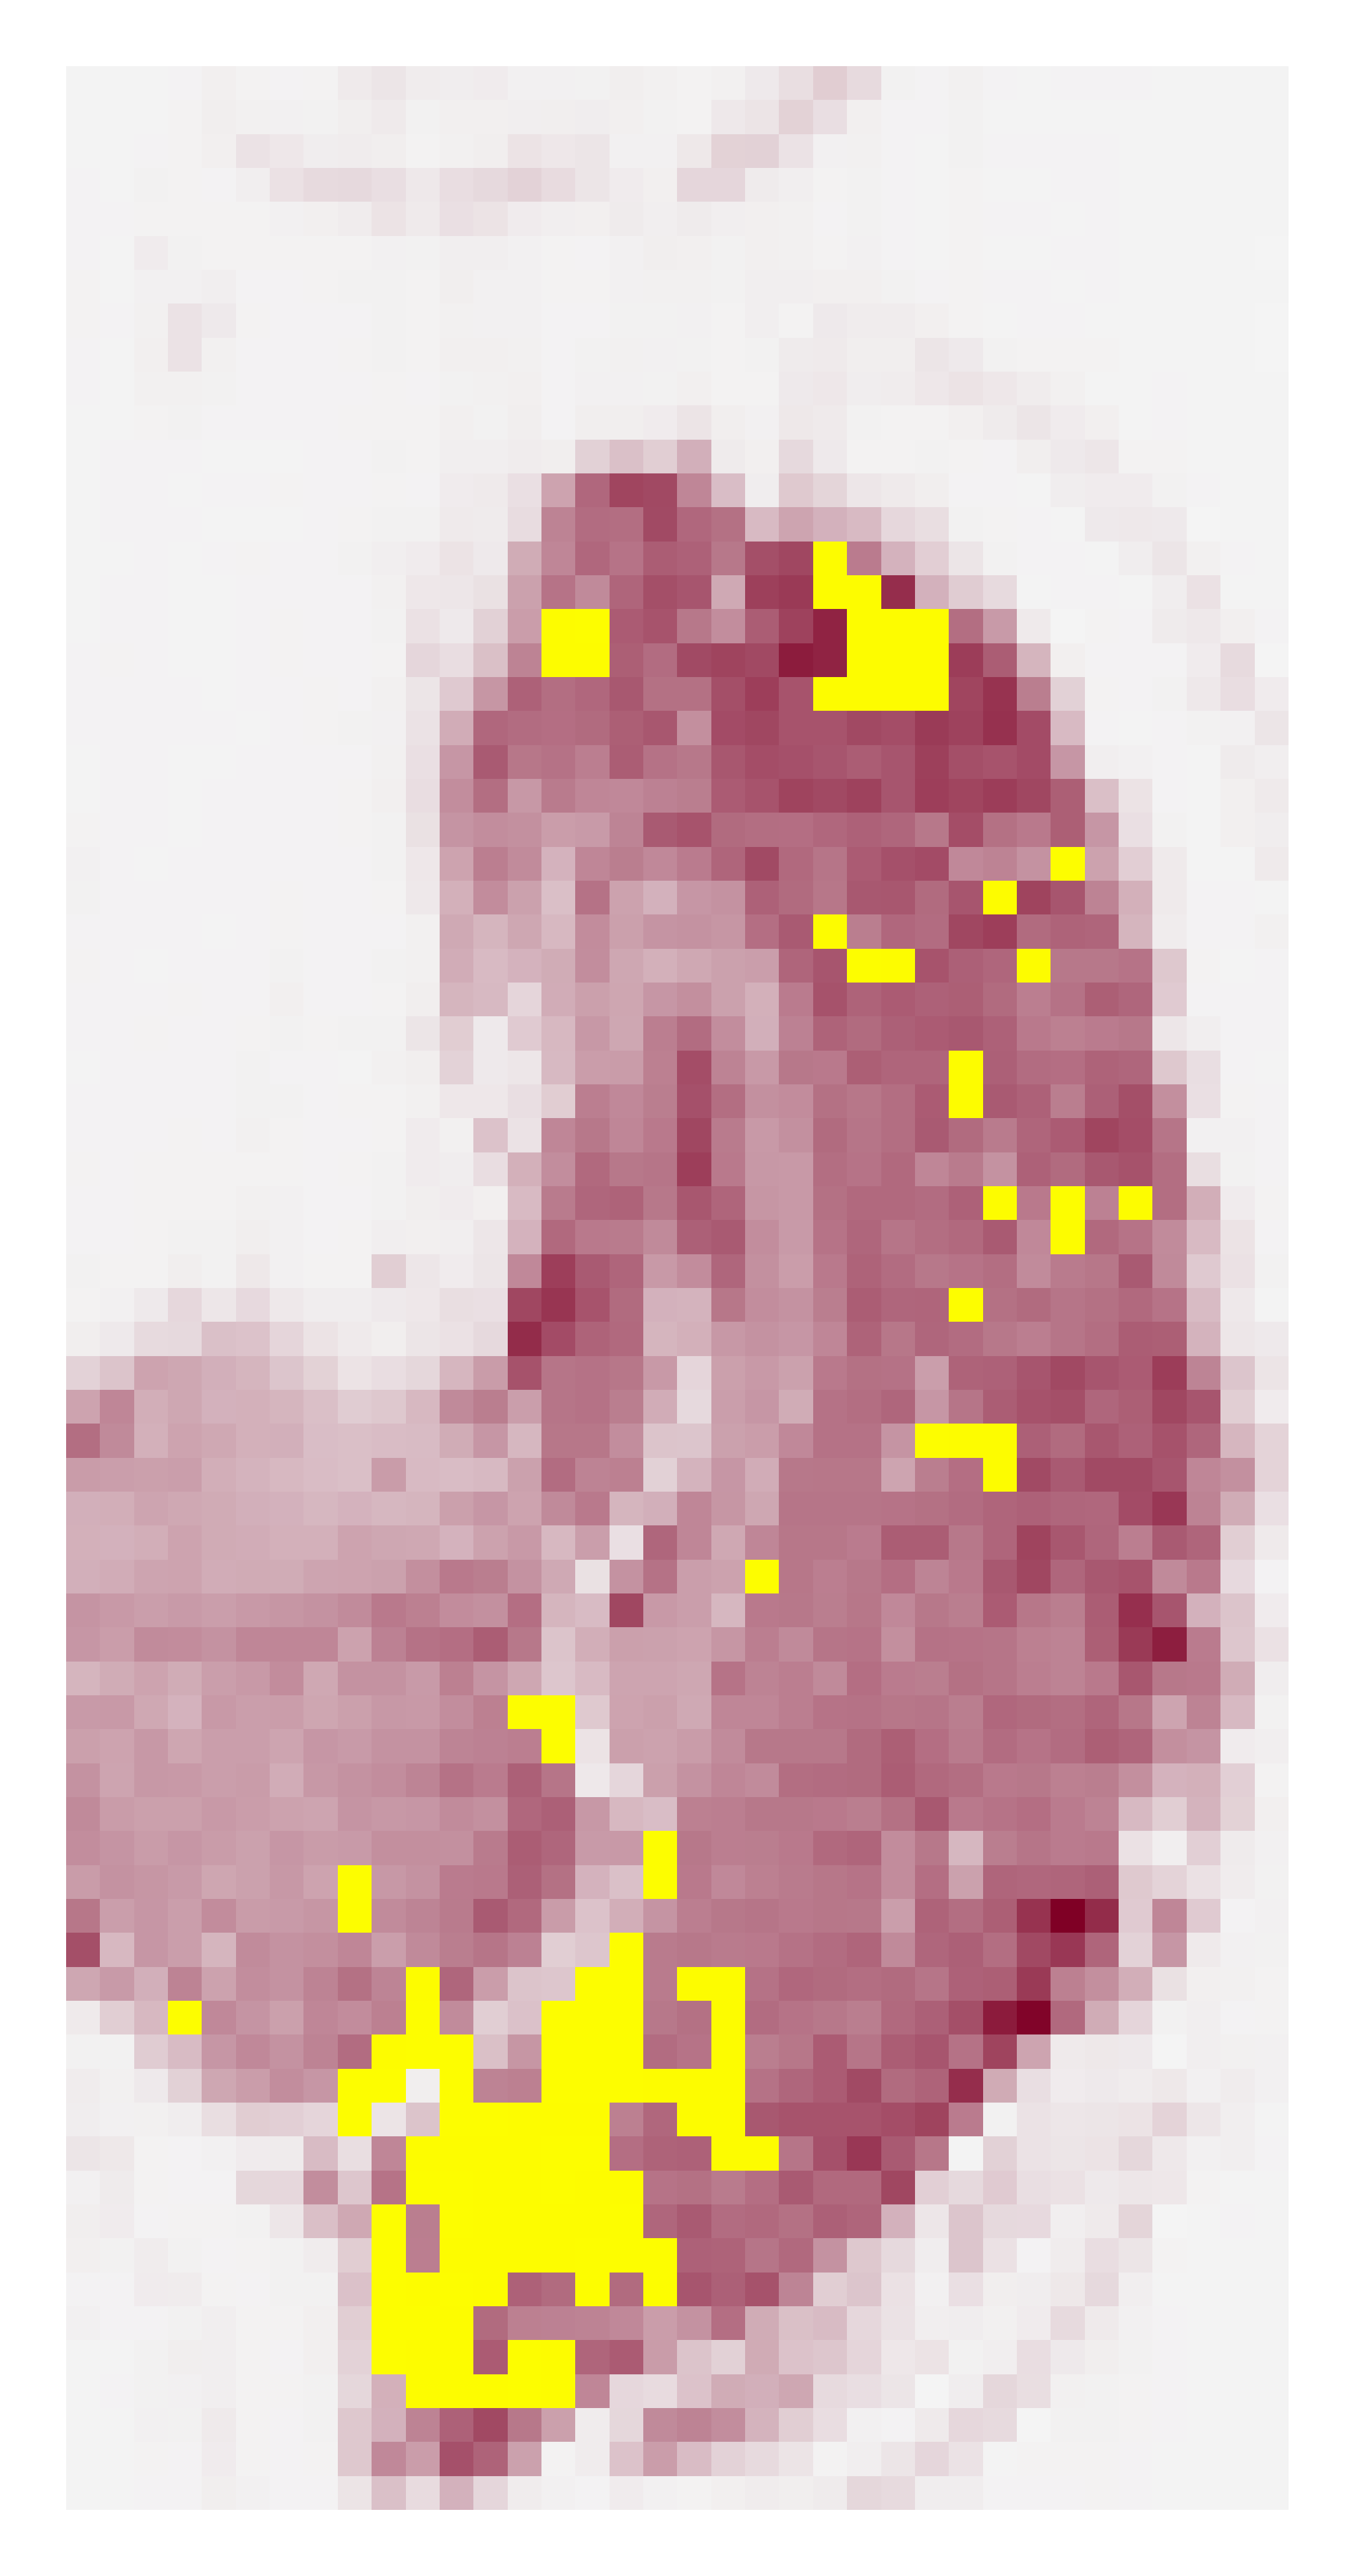
\includegraphics[angle=90]{images/realDataYZ.png}
\caption{$x=36$ Plane of the Activation Regions in Run 1 of Subject 1 During a False Belief Question Stimulus According to \gls{bfast} Algorithm}
\label{fig:realDataYZ}
\end{figure}

\begin{figure}[htbp!]
\centering
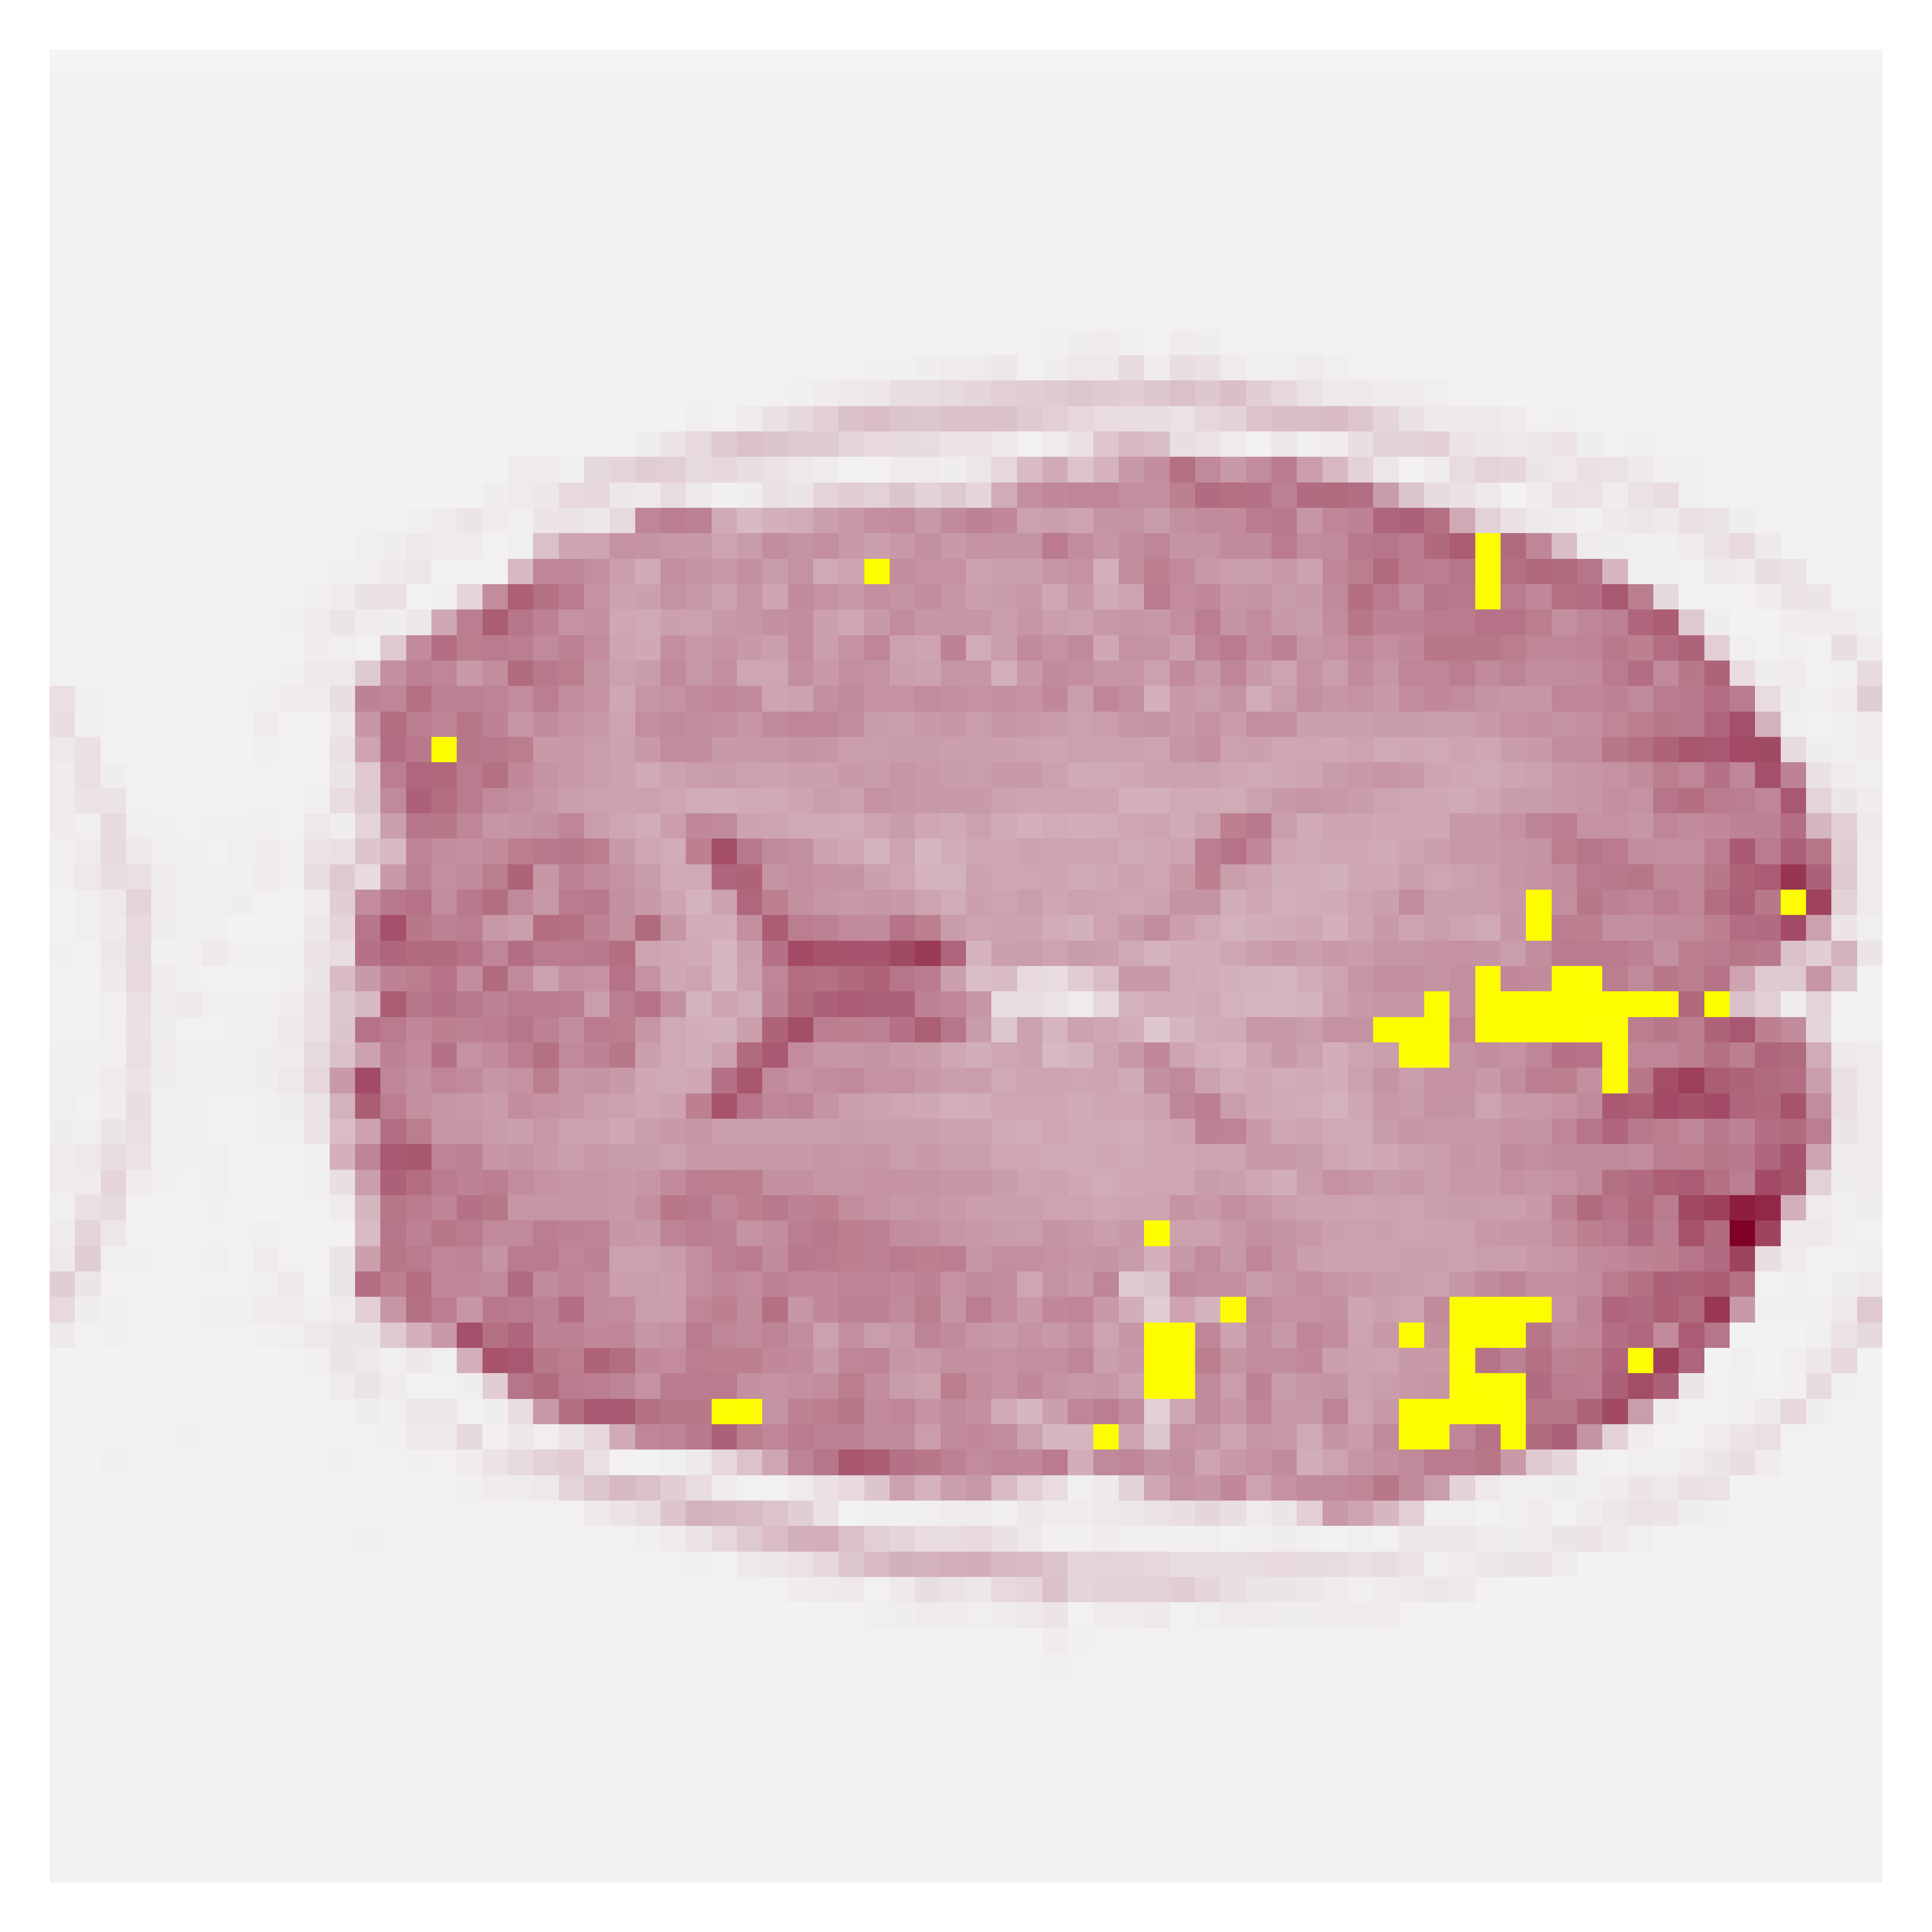
\includegraphics{images/realDataXY.png}
\caption{$z=18$ Plane of the Activation Regions in Run 1 of Subject 1 During a False Belief Question Stimulus According to \gls{bfast} Algorithm}
\label{fig:realDataXY}
\end{figure}